\documentclass[../main.tex]{subfiles}

\begin{document}

\begin{definition}
$C_{pq}$ is a double complex. Filtration by columns $'F_n(Tot(C))$ is the total complex of a truncation of $C$ with $C_{pq}=0$ for $q>n$
\begin{center}
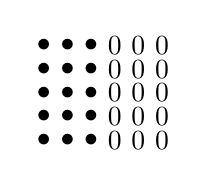
\begin{tikzpicture}[scale=0.3]
\foreach \x in {1,2,3}{
\foreach \y in {-2,-1,...,2}{
\node at (\x,\y) {$0$};
}
}
\foreach \x in {-2,-1,0}{
\foreach \y in {-2,-1,...,2}{
\node at (\x,\y) {$\bullet$};
}
}
\end{tikzpicture}
\end{center}
Filtration by rows $''F_n(Tot(C))$ is the total complex of a truncation of $C$ with $C_{pq}=0$ for $p>n$
\begin{center}
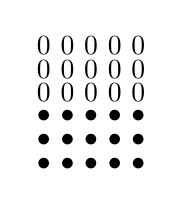
\begin{tikzpicture}[scale=0.3]
\foreach \x in {1,2,3}{
\foreach \y in {-2,-1,...,2}{
\node at (\y,\x) {$0$};
}
}
\foreach \x in {-2,-1,0}{
\foreach \y in {-2,-1,...,2}{
\node at (\y,\x) {$\bullet$};
}
}
\end{tikzpicture}
\end{center}
We have
\['E^0_{pq}=C_{pq}, 'E^1_{pq}=H_q(C_{p*}), 'E^2_{pq}=H^h_pH^v_qC\]
\[''E^0_{pq}=C_{qp}, ''E^1_{pq}=H_q(C_{*p}), 'E^2_{pq}=H^v_qH^h_pC\]
\end{definition}

\end{document}